\documentclass[13pt, letterpaper, oneside]{article}
\usepackage[utf8]{inputenc}
\usepackage[spanish]{babel}
\usepackage{amsmath}
\usepackage{amssymb}
\usepackage{amsfonts}
\usepackage{vmargin}
\usepackage{graphicx}
\usepackage{xcolor}
\usepackage{setspace}
\usepackage{fancyhdr}
\usepackage{titlesec}
\usepackage{lipsum}
\usepackage{geometry}
\usepackage{enumitem}
\usepackage{wrapfig}
\usepackage{subcaption}
\usepackage{url}
\usepackage{float}
\usepackage{datetime}
\usepackage[hidelinks]{hyperref}

\newdateformat{monthyeardate}{%
	\monthname[\THEMONTH], \THEYEAR}
	
\setpapersize{A4}
\setmargins{2.2cm}			%Márgen izquierdo
			{2cm}			%Márgen superior
			{16.5cm}		%Ancho del área de impresión
			{23.42cm}		%Longitud del área de impresión
				{14pt}		%Encabezado
			{5mm}			%Espacio entre el encabezado y el documento
			{2pt}			%Pié de página
			{5mm}			%Espacio entre el pié de página y el documento 
			
\begin{document}

	\include{Carátula}
	
	%--Encabezado y Pié de Página--%
	\pagestyle{fancy}
	\lhead{Síntesis de Redes Activas}
	\rhead{Año 2024}
	\renewcommand{\footrulewidth}{0.08pt}
	
	\tableofcontents
	\pagebreak
	
	\section{Enunciado}
    \subsection{Circuíto 1}
    
    En base a la planilla de requerimientos de la figura 1, se pide:\\
    
    \begin{itemize}
        \item Aproximar la función de atenuación, mediante polinomios de \textbf{chebychev} utilizando como herramiento python o matlab.\\
        \item Sintetizar un circuíto que satisfaga los requerimientos del punto anterior utilizando topologías bicuadráticas de realimentación positiva o negativa (a elección).\\
        \item Simular cada etapa y el filtro total en LTSPICE.\\
        \item Calcular la sensibilidad de la frecuencia del polo de cada bicuadrática ($\omega_p$) y del ancho de banda ($\omega_p/Q_p$).\\
        \item Analizar la desviación si todos los elementos tienen una tolerancia del 10%.\\
        \item Realizar una simulación de Montecarlo de las desviaciones con LTSPICE.\\
        \item Armar el circuíto, medir experimentalmente las curvas de atenuación y defasaje. Contrastarlas con lo teórico y las simulaciones.
    \end{itemize}
    
    \begin{figure}[ht]
        \centering
        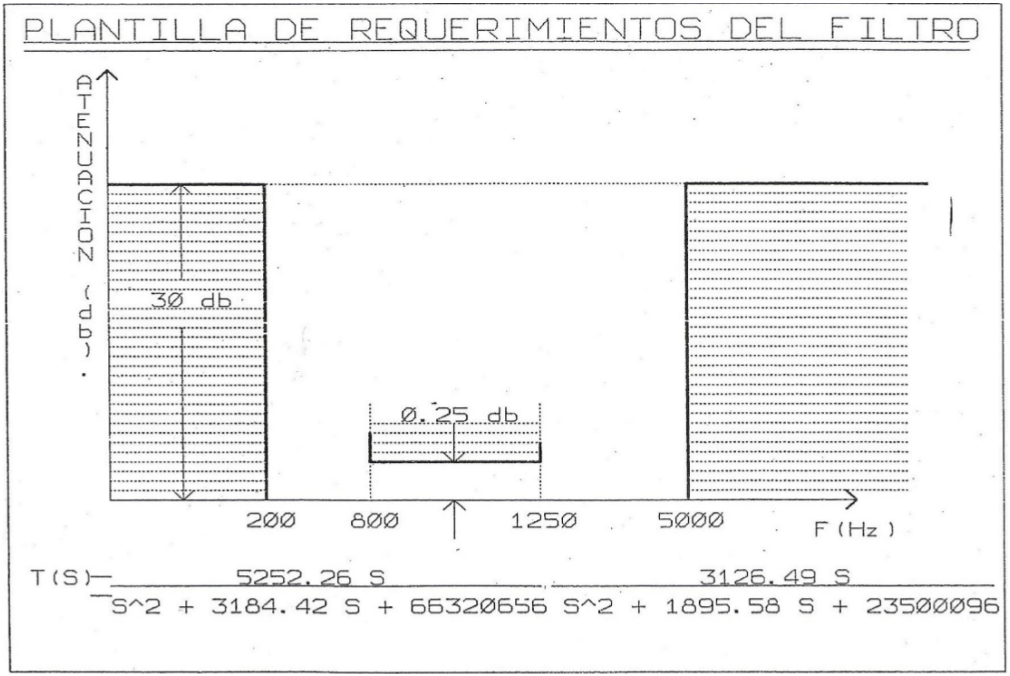
\includegraphics[height=8cm]{Imágenes/Req.png}
        \caption{Requerimientos del filtro}
    \end{figure}

    \newpage
    \subsection{Metodología}
    En general, para cada uno de los casos particulares solicitados se debe.\\
    \begin{itemize}
        \item  Realizar una sintética introducción teórica.
        \item  Analizar el circuíto propuesto, su desarrollo numérico y todos los cálculos analíticos.
        \item Realizar simulaciones en LTSPICE.
        \item Armar el circuíto y hacer las mediciones en laboratorio.
        \item Finalmente, compara los valores calculados, simulados y medidos, y extraer conclusiones acerca de las diferencias. Analizar las causas.
        \item Presentar un informe digital y en papel.
    \end{itemize}
    \newpage

\section{Introducción}
    Aquí se presentará una breve introducción teórica del tema a desarrollar.\\
    Características principales de los polinomios de Chebyshev en el diseño de los filtros.\\

    \begin{itemize}
        \item \textbf{Atenuaciones Específicas}: Estos polinomios permiten diseñar los filtros con características determinadas de atenuación en la banda de paso. Esto significa que es posible lograr grandes atenuaciones con respecto a otros polinomios como los de Butterworth.
        \item \textbf{Orden Bajo}: Estos polinomios permiten minimazar el orden con mayores atenuaciones, esto permite que los mismos tengan un menor coste y sean más fáciles de implementar.
        \item \textbf{Optimización del ancho de banda}: Estos polinomios permiten optimizar el ancho de banda del filtro manteniendo la misma atenuación en la banda de paso.
        \item \textbf{Flexibilidad del diseño}: Permiten ajustar los parámetros del filtro tales como la atenuación máxima en la banda de paso y la frecuencia de corte, satisfaciendo los requerimientos dados.
    \end{itemize}

\newpage
\section{Desarrollo}
    De acuerdo a lo especificado en la plantilla de requerimientos podemos extraer del mismo la siguiente información:\\

    \begin{itemize}
        \item Banda de Paso: Desde 800 hasta 1250 [Hz] con una atenuación máxima de 0.25 [dB].
        \item Banda de Rechazo: Menores a 200 y mayores a 5000 [Hz] con una atenuación mínima de 30 [dB].
    \end{itemize}

    Con estos criterios dados, utilizaremos python para sintetizar el filtro de la siguiente manera:\\

    Para ello, colocamos las especificaciones dadas como parámetros de entrada.\\

    \begin{figure}[ht]
        \centering
        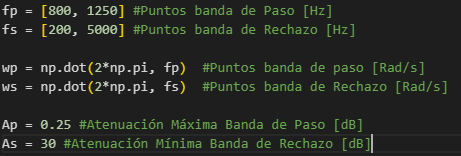
\includegraphics[height=4cm]{Imágenes/Descrip.png}
        \caption{Especificaciones}
    \end{figure}

    Lugo, utilizaremos la librería \textbf{scipy} para obtener el polinomio de chebyshev de la siguiente manera, además utilizaremos la librería \textbf{control} para colocarlo de forma de función de transferencia y lograr hacer el diagrama de bode de una manera más sencilla:\\
    
    \begin{figure}[ht]
        \centering
        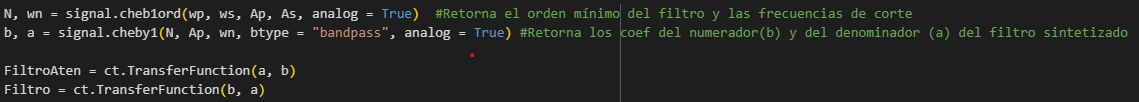
\includegraphics[height=1.5cm]{Imágenes/Descrip2.png}
        \caption{Obtención del polinomio}
    \end{figure}

    Con esto podemos graficar la respuesta en bode (En atenuación) para compararla con lo espeficicado.\\
    
    \begin{figure}[ht]
        \centering
        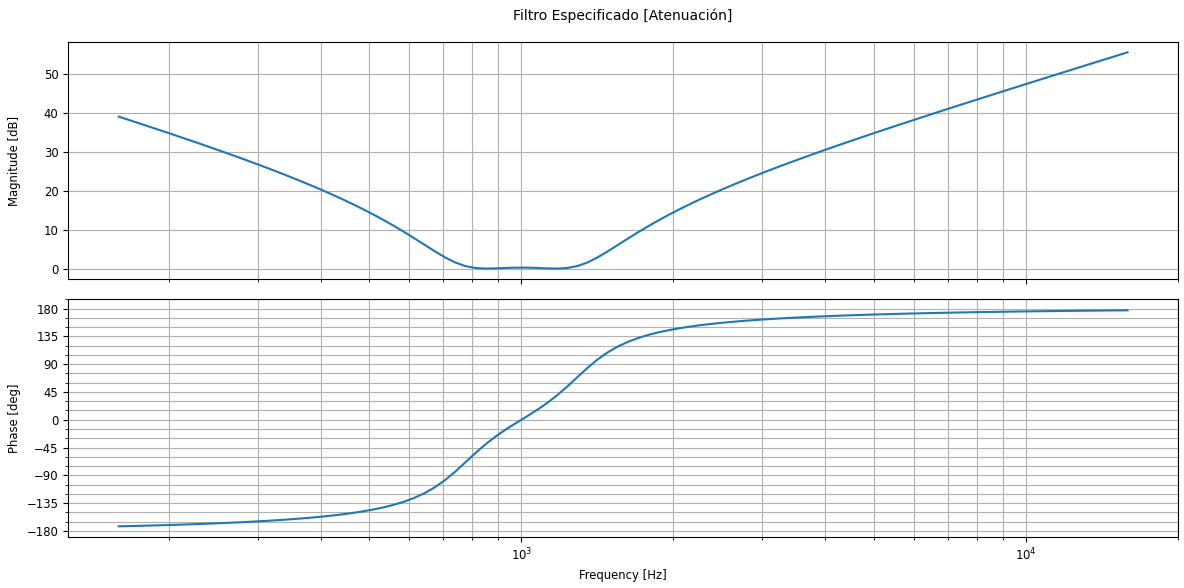
\includegraphics[height=9cm]{Imágenes/filtro.png}
        \caption{Bode del filtro}
    \end{figure} 

    \newpage

    La función de transferencia dada del filtro, será la siguiente:\\

    \begin{figure}[ht]
        \centering
        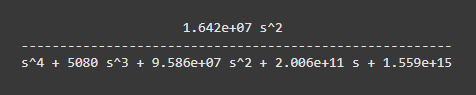
\includegraphics[height=2.5cm]{Imágenes/ft.png}
        \caption{Función de Transferencia}
    \end{figure} 

    Se aprecia que el filtro tiene un comportamiento de pasa banda, es por eso que podemos separarlo en dos filtros, un pasa alto y un pasa bajo, de manera que sea posible sintetizarlo mediante topologías bicuadráticas.\\

    Para la topología de un filtro pasa bajo, se obtiene la siguiente función de transferencia:\\
    \begin{figure}[ht]
        \centering
        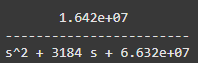
\includegraphics[height=2.5cm]{Imágenes/PasaBajo.png}
        \caption{Pasa Bajo}
    \end{figure} 

    En cambio, para la topología de un filtro pasa alto, se obtiene la siguiente función de transferencia:\\
    \begin{figure}[ht]
        \centering
        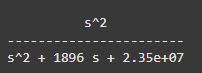
\includegraphics[height=2.5cm]{Imágenes/PasaAlto.png}
        \caption{Pasa Alto}
    \end{figure} 

    \newpage
    Si graficamos la respuesta en frecuencia de cada bicuadrática y el conjunto de las mismas, vemos que se responde correctamente a lo especificado:\\
    \begin{figure}[ht]
        \centering
        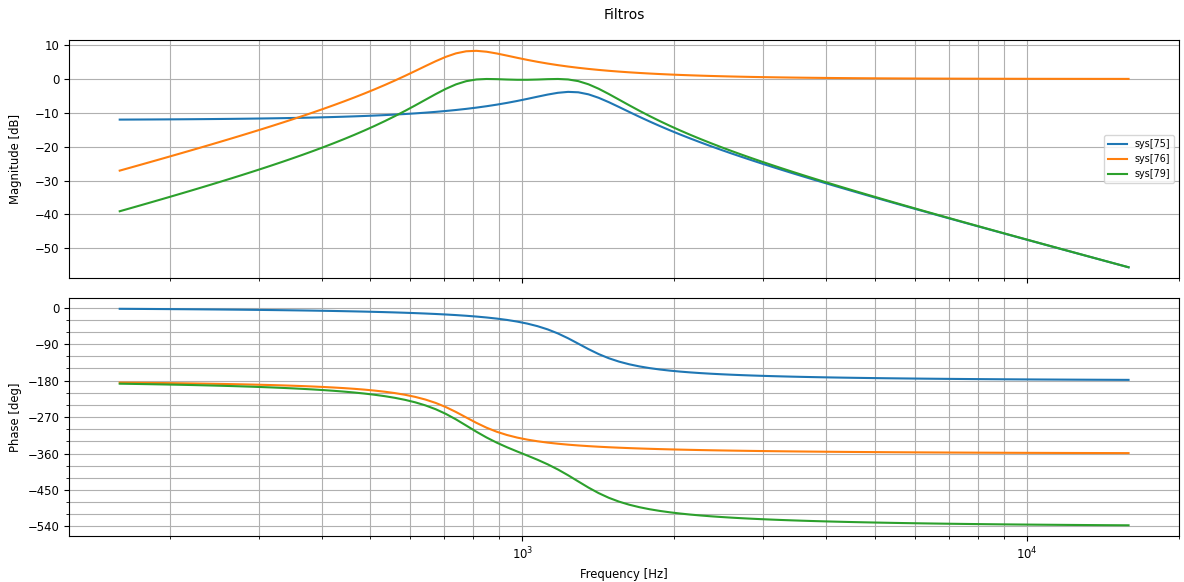
\includegraphics[height=9cm]{Imágenes/Filtros.png}
        \caption{Respuesta en Frecuencia}
    \end{figure}

    \newpage
    \subsection{Pasa Alto}
    \subsubsection{Síntesis}
    Para sintetizar esta bicuadrática, se utilizará la topología de realimentación positiva "Sallen key". La función de transferencia a lograr es la siguiente:\\

    \begin{center}
        \boxed{\frac{s^2}{s^2 + 1896*s + 2.35*10^7}}
    \end{center}

    El circuíto modelo a utilizar y calcular es el siguiente:\\

    \begin{figure}[ht]
        \centering
        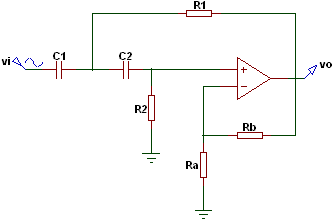
\includegraphics[height=8cm]{Imágenes/Alto.png}
        \caption{Sallen Key Pasa Alto}
    \end{figure}

    Con este circuíto, se plantea el siguiente sistema de ecuaciones en base a la siguiente red y planteando que el amplificador operacional es ideal y no posee polos que modifiquen la respuesta del filtro:\\

    \begin{figure}[ht]
        \centering
        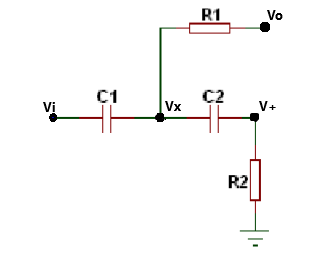
\includegraphics[height=5cm]{Imágenes/RedAlta.png}
        \caption{Red Pasa Alto}
    \end{figure}

    \newpage
    Utilizando el método de nodos se plantea el \textbf{Sistema de Ecuaciones} dado:\\
    
    \begin{itemize}
        \item $V_i*sC_1 + V_o*\frac{1}{R_1} = V_x*(sC_1+sC_2+\frac{1}{R_1}) - V_+*(sC_2)$
        \item $0 = -V_x*(sC_2) +V_+*(\frac{1}{R_2} + sC_2)$
    \end{itemize}

    Si resolvemos para determinar $V_+$, nos quedará la siguiente solución, haciendo que $C_1 = C_2 = C$:\\

    \begin{center}
        $V_+ = \frac{V_i*(s^2C^2) + V_o*(s\frac{C}{R_1})}{s^2C^2 + sC(\frac{2}{R_2}+\frac{1}{R_1})+\frac{1}{R_2R_1}}$
    \end{center}

    Donde podemos identificar:\\
    
    \begin{itemize}
        \item $D = s^2C^2 + sC(\frac{2}{R_2}+\frac{1}{R_1})+\frac{1}{R_2R_1}$
        \item $N_{ff} = s^2C^2$
        \item $N_{fb} = s\frac{C}{R_1}$
    \end{itemize}

    Ahora $k = \frac{R_a + R_b}{Ra}$ y la solución del filtro es:\\

    \begin{center}
        \large{$\frac{V_o}{V_i} = \frac{k.N_{ff}}{D-k.N_{fb}} = \frac{k.s^2C^2}{s^2C^2 + sC(\frac{2}{R_2}+\frac{1}{R_1})+\frac{1}{R_2R_1} - k.s\frac{C}{R_1}}$}
    \end{center}

    Si expresamos de otra forma e igualamos a nuestra función de transferencia deseada:\\

    \begin{center}
        \boxed{\frac{s^2}{s^2 + 1896*s + 2.35*10^7} = \frac{k.s^2}{s^2 + \frac{s}{C}.(\frac{2}{R_2} + \frac{1-k}{R_1}) + \frac{1}{R_1R_2C^2}}}
    \end{center}

    Por lo que la solución al sistema, planteando que $k=1$, serán los siguientes componentes pasivos:\\

    \begin{itemize}
        \item $C_1 = C_2 = 1 [F] \xrightarrow{} 1 [uF]$
        \item $R_1 = 40.34 [u\Omega] \xrightarrow{} 40.34 [\Omega]$
        \item $R_2 = 1.055 [m\Omega] \xrightarrow{} 1.055 [k\Omega]$
    \end{itemize}

    Para que $k=1$ entonces, el AO deberá ser colocado como un buffer.\\
    \newpage
    \subsubsection{Simulaciones}
    Simularemos el siguiente circuíto con la topología dada y los elementos pasivos ya calculados:\\

    \begin{figure}[ht]
        \centering
        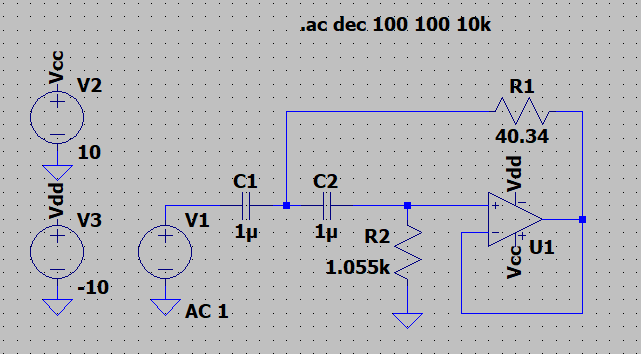
\includegraphics[height=6cm]{Imágenes/spiceAlto.png}
        \caption{Circuíto Simulado}
    \end{figure}
    
    \begin{figure}[ht]
        \centering
        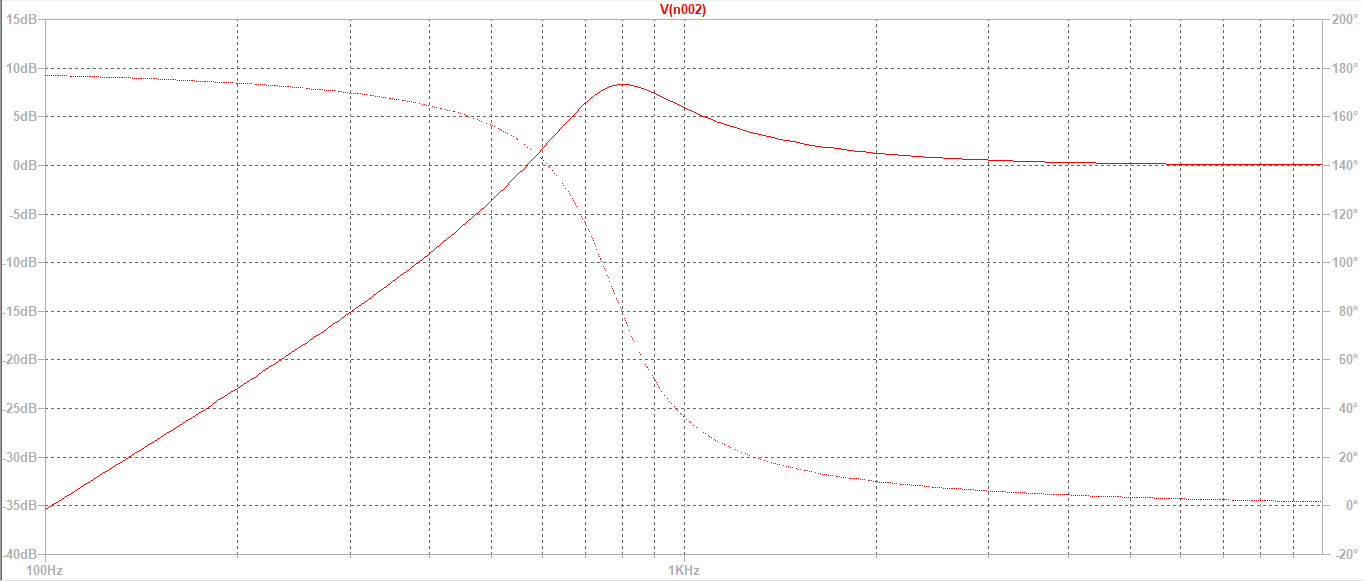
\includegraphics[height=7cm]{Imágenes/BodeAlto.png}
        \caption{Bode Filtro Pasa Alto}
    \end{figure}
    
    
    \newpage
    \subsection{Pasa Bajo}
    \subsubsection{Síntesis}
    Para sintetizar esta bicuadrática, también se utilizará la topología de realimentación positiva "Sallen key". La función de transferencia a lograr es la siguiente:\\

    \begin{center}
        \boxed{\frac{1.642*10^7}{s^2 + 3184*s + 6.632*10^7}}
    \end{center}

    El circuíto modelo a utilizar y calcular es el siguiente:\\

    \begin{figure}[ht]
        \centering
        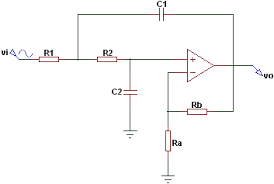
\includegraphics[height=7cm]{Imágenes/Bajo.png}
        \caption{Sallen Key Pasa Bajo}
    \end{figure}

    Con este circuíto, se plantea el siguiente sistema de ecuaciones en base a la siguiente red y planteando que el amplificador operacional es ideal y no posee polos que modifiquen la respuesta del filtro:\\

    \begin{figure}[ht]
        \centering
        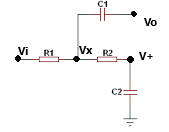
\includegraphics[height=5cm]{Imágenes/RedBajo.png}
        \caption{Red Pasa Bajo}
    \end{figure}

    \newpage
    Utilizando el método de nodos se plantea el \textbf{Sistema de Ecuaciones} dado, haciendo que $C_1 = C_2 = C$ y $R_1 = R_2 = R$:\\
    
    \begin{itemize}
        \item $\frac{V_i}{R}+V_o.sC =V_x.(\frac{2}{R}+sC) - V_+.(\frac{1}{R})$
        \item $0 = -V_x.(\frac{1}{R}) + V_+.(\frac{1}{R} + sC)$
    \end{itemize}

    Si resolvemos para determinar, obtendremos la siguiente expresión:\\

    \begin{center}
        $V_+ = \frac{V_i + V_o.sCR}{s^2C^2R^2+3SCR + 1}$
    \end{center}

    Donde podemos identificar:\\
    
    \begin{itemize}
        \item $D = s^2C^2R^2+3SCR + 1$
        \item $N_{ff} = 1$
        \item $N_{fb} = sCR$
    \end{itemize}

    Ahora $k = \frac{R_a + R_b}{Ra}$ y la solución del filtro es:\\

    \begin{center}
        \large{$\frac{V_o}{V_i} = \frac{k.N_{ff}}{D-k.N_{fb}} = \frac{k}{s^2C^2R^2+3SCR + 1-k.sCR} = \frac{k}{s^2C^2R^2+SCR(3-k) + 1}$}
    \end{center}

    Si expresamos de otra forma e igualamos a nuestra función de transferencia deseada:\\

    \begin{center}
        \boxed{\frac{1.642*10^7}{s^2 + 3184*s + 6.632*10^7} = \frac{k.\frac{1}{C^2R^2}}{s^2 + s\frac{3-k}{CR} + \frac{1}{C^2R^2}}}
    \end{center}

    Ahora:\\
    
    \begin{center}
        $CR = 122.79.10^-6$\\
        $k = 2.609$\\
    \end{center}

    Si hago que $C=1[F]$ para luego escalar, entonces:\\

    \begin{itemize}
        \item $C_1 = C_2 = 1 [F] \xrightarrow{} 0.1 [uF]$
        \item $R_1 = R_2 = 122.79 [u\Omega] \xrightarrow{} 1.228 [K\Omega]$
    \end{itemize}

    Esto nos dará la siguiente función de transferencia, la cual tendremos que escalar para obtener la esperada.\\

    \begin{center}
        $\frac{173.01*10^6}{s^2 + 3184 + 6.632*10^7}$
    \end{center}

    El factor de escala será de $G = 0.094908$, esto lo podemos lograr mediante un divisor resistivo a la entrada de la red atenuando para lograr lo requerido, es posible sólo agregando una resistencia adicional y mediante thevenin, teniendo en cuenta que:\\

    \begin{itemize}
        \item $R_1 = R_3//R_4 = 1.228 [k\Omega]$
        \item $G = 0.094908 = \frac{R_4}{R_4+R_3}$
    \end{itemize}

    Resolviendo este sistema de ecuaciones:\\

    \begin{itemize}
        \item $R_3 = 1.3568 [k\Omega]$
        \item $R_4 = 12.939 [k\Omega]$
    \end{itemize}

    Además para obtener el k deseado:\\

    \begin{itemize}
        \item $R_a = 621.5 [\Omega]$
        \item $R_b = 1 [k\Omega]$
    \end{itemize}
    
    \newpage
    \subsubsection{Simulaciones}
    Simularemos el siguiente circuíto con la topología dada y los elementos pasivos ya calculados:\\

    \begin{figure}[ht]
        \centering
        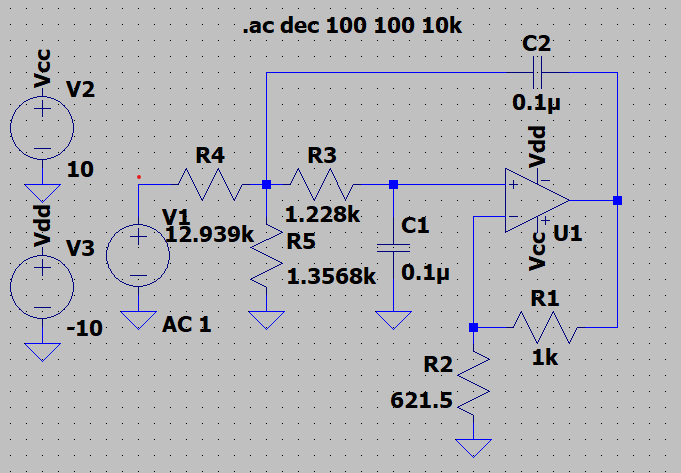
\includegraphics[height=6cm]{Imágenes/spiceBajo.png}
        \caption{Circuíto Simulado}
    \end{figure}
    
    \begin{figure}[ht]
        \centering
        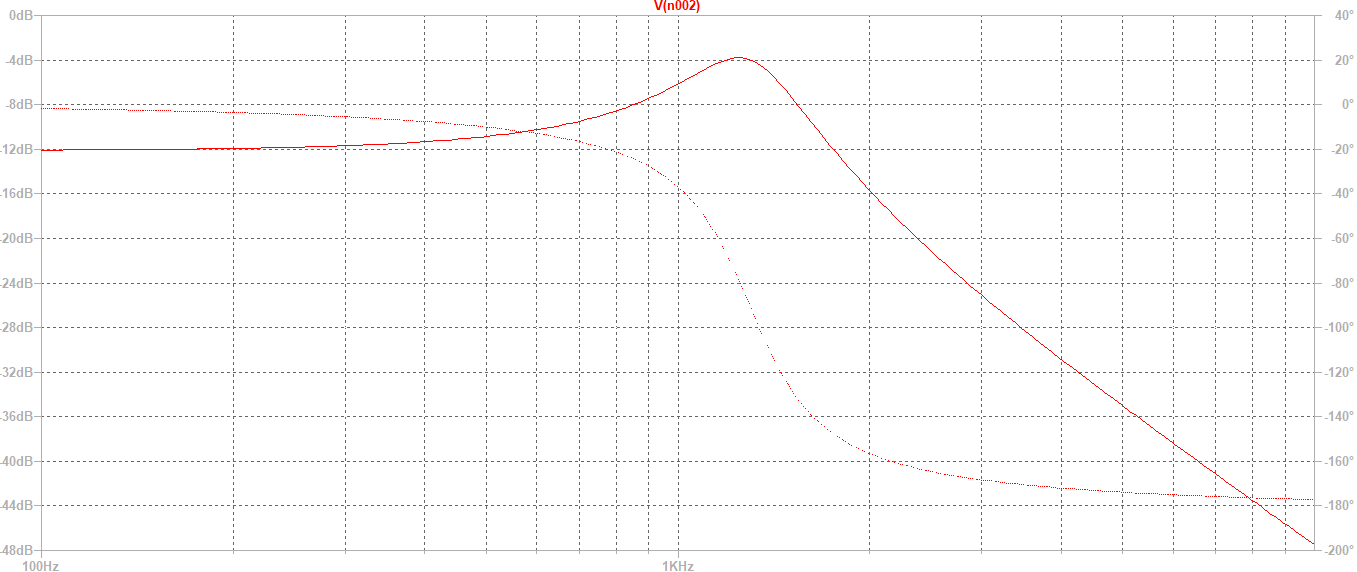
\includegraphics[height=7cm]{Imágenes/BodeBajo.png}
        \caption{Bode Filtro Pasa Bajo}
    \end{figure}
    
    
    \newpage
    \subsection{Filtro Completo}
    Para la realización del filtro completo, tan sólo es necesario conectar ambos circuitos ya calculados de forma salida-entrada.\\
    
    \subsubsection{Simulaciones}

    \begin{figure}[ht]
        \centering
        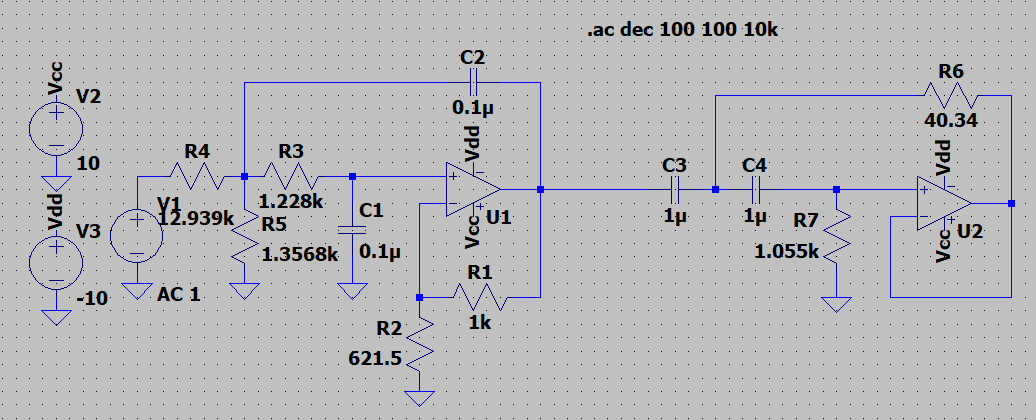
\includegraphics[height=6cm]{Imágenes/spiceCompleto.png}
        \caption{Circuíto Simulado}
    \end{figure}
    
    \begin{figure}[ht]
        \centering
        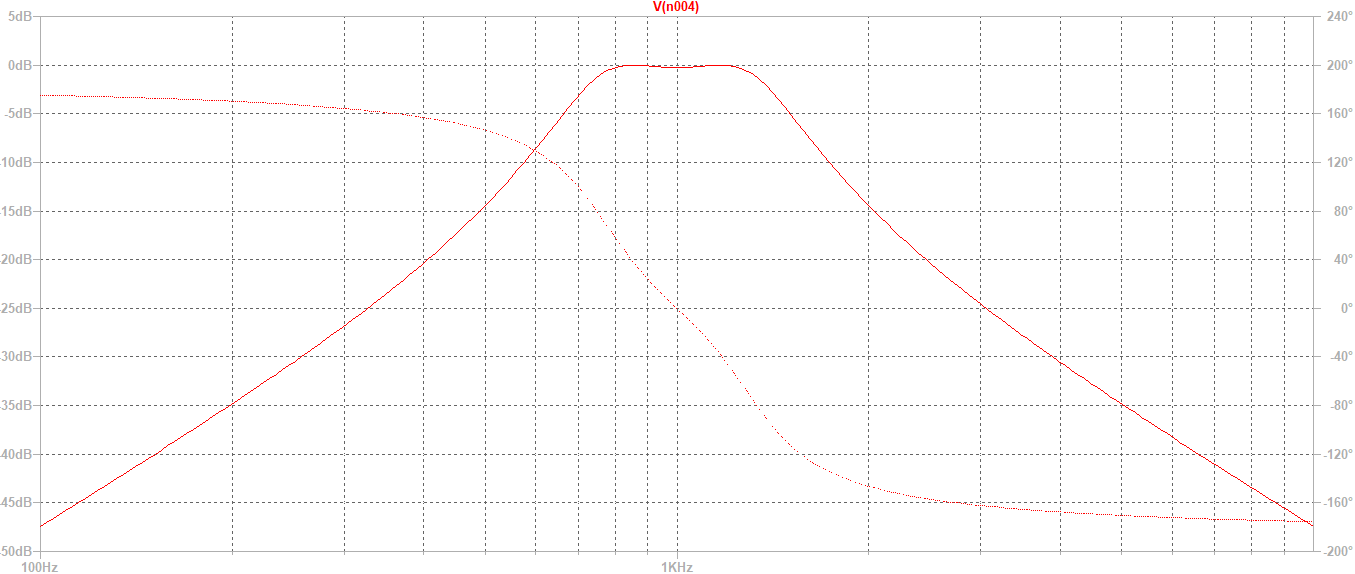
\includegraphics[height=7cm]{Imágenes/BodeCompleto.png}
        \caption{Bode Filtro Pasa Banda}
    \end{figure}

    Realizando un ajuste a las frecuencias de importancia y determinando mediante cursores:\\

    \begin{itemize}
        \item $800[Hz]: -0.257 [dB]$
        \item $1250[Hz]: -0.266 [dB]$
        \item $200[Hz]: -34.8 [dB]$
        \item $5000[Hz]: -34.88 [dB]$
    \end{itemize}

    Podemos comprobar que este filtro cumple con lo especificado.\\
    
    
    \subsubsection{Sensibilidad}
    Para calcular la sensibilidad de la frecuencia de los polos $\omega_p$ y el ancho de banda $(\omega_p/Q_p)$, se toma las expresiones dadas anteriormente para cada caso (bicuadrática), donde:\\

    \Large{\textbf{Pasa Bajo}}
    
    \begin{center}
        \boxed{\frac{\omega_p^2}{s^2+\frac{\omega_p}{Q_p}.s+\omega_p^2} = \frac{k.\frac{1}{C^2R^2}}{s^2 + s\frac{3-k}{CR} + \frac{1}{C^2R^2}}}
    \end{center}

    Siendo entonces:\\

    \begin{itemize}
        \item $\omega_p = \frac{1}{CR}$
        \item $\omega_p/Q_p = \frac{3-k}{CR}$
    \end{itemize}

    Siendo $k = \frac{R_a + R_b}{Ra}$.\\

    Entonces:\\

    \begin{center}
        $S(\frac{\omega_p}{R}) = \frac{R.\partial\omega_p}{\omega_p.\partial R} = -1$\\
        
        $S(\frac{\omega_p}{C}) = \frac{C.\partial\omega_p}{\omega_p.\partial C} = -1$\\
        
        $S(\frac{\omega_p}{k}) = \frac{k.\partial\omega_p}{\omega_p.\partial k} = 0$\\
        
        $S(\frac{\omega_p/Q_p}{R}) = \frac{R.\partial(\omega_p/Q_p)}{(\omega_p/Q_p).\partial R} = 0$\\
        
        $S(\frac{\omega_p/Q_p}{C}) = \frac{C.\partial(\omega_p/Q_p)}{(\omega_p/Q_p).\partial C} = 0$\\

        $S(\frac{\omega_p/Q_p}{k}) = \frac{k.\partial(\omega_p/Q_p)}{(\omega_p/Q_p).\partial k} = \frac{-k}{k-3} = 6.67$\\
    \end{center}    

    Se desarrollará una tabla para determinar las variaciones y ajustar tolerancias de los componentes, asegurando la mínima desviación posible, Además se procederá a colocar valores comerciales de componentes con su respectiva serie.\\

    \begin{figure}[ht]
        \centering
        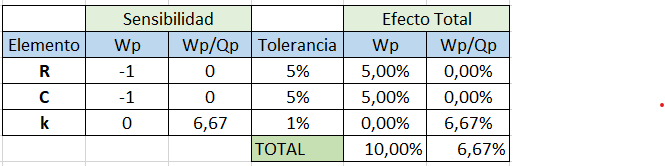
\includegraphics[height=5cm]{Imágenes/SensBajo.png}
        \caption{Variación de los parámetros Pasa Bajo}
    \end{figure}

    \newpage
    \Large{\textbf{Pasa Alto}}
    
    \begin{center}
        \boxed{\frac{s^2}{s^2+\frac{\omega_p}{Q_p}.s + \omega_p^2} = \frac{k.s^2}{s^2 + \frac{s}{C}.(\frac{2}{R_2} + \frac{1-k}{R_1}) + \frac{1}{R_1R_2C^2}}}
    \end{center}
    
    Siendo entonces:\\

    \begin{itemize}
        \item $\omega_p = \frac{1}{C\sqrt{R_1R_2}}$
        \item $\omega_p/Q_p = \frac{2R_1+R_2.(1-k)}{C.R_1.R_2}$
    \end{itemize}

    Siendo $k = \frac{R_a + R_b}{Ra}$.\\

    Entonces:\\

    \begin{center}
        $S(\frac{\omega_p}{R_1}) = \frac{R_1.\partial\omega_p}{\omega_p.\partial R_1} = -0.5$\\
        
        $S(\frac{\omega_p}{R_2}) = \frac{R_2.\partial\omega_p}{\omega_p.\partial R_2} = -0.5$\\
        
        $S(\frac{\omega_p}{C}) = \frac{C.\partial\omega_p}{\omega_p.\partial C} = -1$\\

        $S(\frac{\omega_p}{k}) = \frac{k.\partial\omega_p}{\omega_p.\partial k} = 0$\\
        
        $S(\frac{\omega_p/Q_p}{R_1}) = \frac{R_1.\partial(\omega_p/Q_p)}{(\omega_p/Q_p).\partial R_1} = \frac{R_2.(k-1)}{2.R_1-(k-1).R_2} = 0$\\
        
        $S(\frac{\omega_p/Q_p}{R_2}) = \frac{R_2.\partial(\omega_p/Q_p)}{(\omega_p/Q_p).\partial R_2} = \frac{2.R_1}{R_2.(k-1)-2.R_1} = -1$\\

        $S(\frac{\omega_p/Q_p}{C}) = \frac{C.\partial(\omega_p/Q_p)}{(\omega_p/Q_p).\partial C} = -1$\\

        $S(\frac{\omega_p/Q_p}{k}) = \frac{k.\partial(\omega_p/Q_p)}{(\omega_p/Q_p).\partial k} = \frac{k.R_2}{k.R_2-2.(R_1+0.5.R_2)} = -13.076$\\
    \end{center}  

    De la misma manera, desarrollamos una tabla:\\

    \begin{figure}[ht]
        \centering
        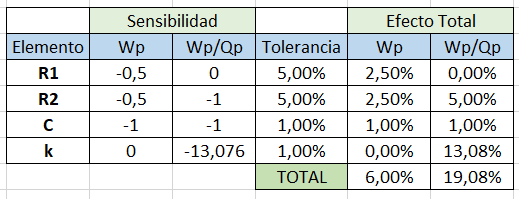
\includegraphics[height=5cm]{Imágenes/SensAlto.png}
        \caption{Variación de los parámetros Pasa Alto}
    \end{figure}

    \newpage
    \subsubsection{Análisis de Montecarlo}
    
    Para este análisis se colocarán los valores comerciales de los componentes pasivos con las tolerancias dadas anteriormente.\\

    \begin{figure}[ht]
        \centering
        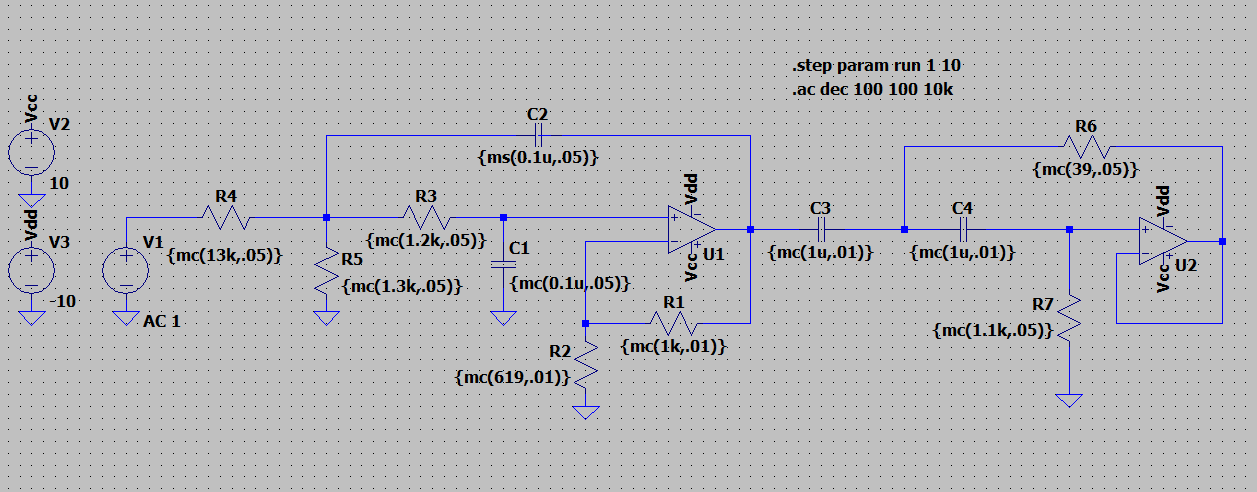
\includegraphics[height=5cm]{Imágenes/completo.png}
        \caption{Circuíto a Simular}
    \end{figure}

    \begin{figure}[ht]
        \centering
        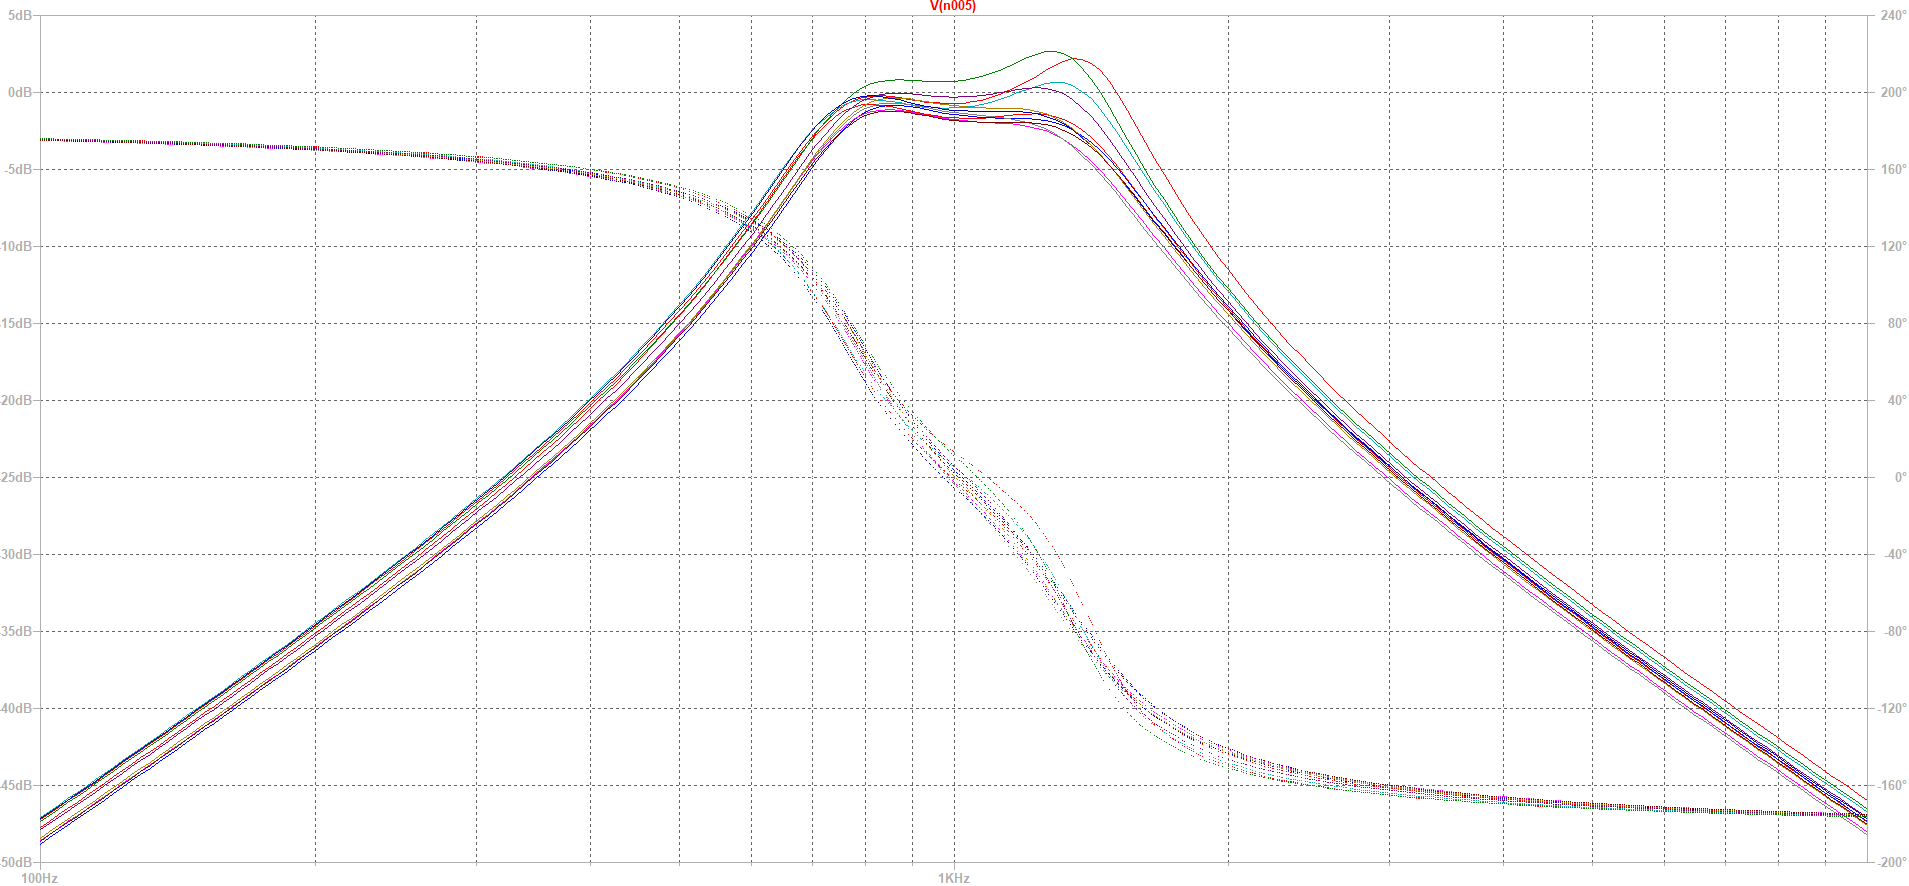
\includegraphics[height=8cm]{Imágenes/montecarlo.png}
        \caption{Simulación Monte-Carlo}
    \end{figure}

    \begin{figure}[ht]
        \centering
        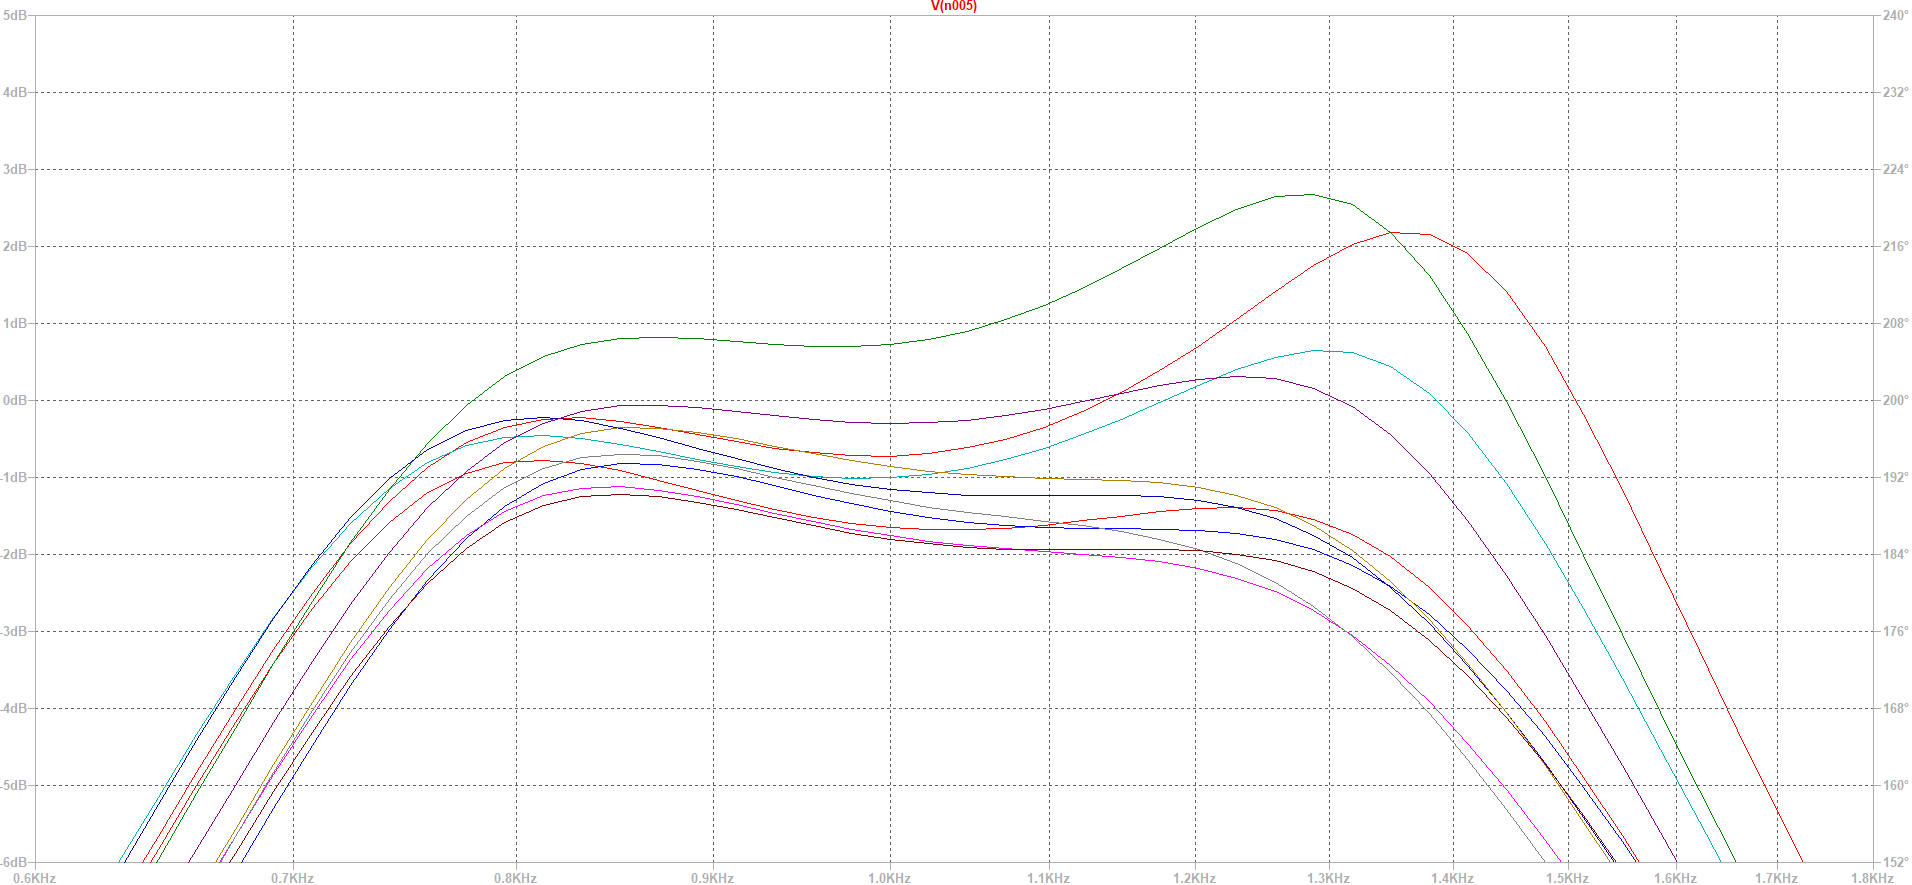
\includegraphics[height=8cm]{Imágenes/montecarlo2.png}
        \caption{Zoom Monte-Carlo}
    \end{figure}
    
	
\end{document}
